\documentclass[10pt,a4paper]{article}
\usepackage[T1]{fontenc}
\usepackage[utf8]{inputenc}
\usepackage{mathptmx}
\usepackage[margin=24mm]{geometry}
\usepackage{microtype,amsmath,amssymb,booktabs,tabularx,array}
\usepackage{tikz}
\usetikzlibrary{arrows.meta,positioning,calc}
\usepackage{float,caption,enumitem,fancyhdr}
\usepackage{graphicx}
\usepackage{titlesec}
\titlespacing*{\section}{0pt}{12pt}{6pt}
\titlespacing*{\subsection}{0pt}{9pt}{4pt}
\usepackage{hyperref}
\hypersetup{pdftitle={MAC Table Flooding and Fair-Eviction Defense - Final Report},pdfauthor={2105085 and 2105062},colorlinks=true,linkcolor=blue,urlcolor=blue,citecolor=blue}
\newcounter{algctr}
\newenvironment{algobox}[1]{%
\begin{figure}[H]\refstepcounter{algctr}\centering
\begin{minipage}{\linewidth}
\noindent\rule{\linewidth}{0.7pt}\\[2pt]
\textbf{Algorithm \thealgctr.} #1\\[3pt]
\noindent\rule{\linewidth}{0.4pt}\vspace{4pt}\par
\small
}{%
\vspace{2pt}\noindent\rule{\linewidth}{0.7pt}
\end{minipage}
\end{figure}
}
\setlength{\parindent}{1.2em}
\setlength{\parskip}{2pt}
\setlength{\headheight}{14pt}
\setlist{nosep,leftmargin=*}
\captionsetup{font=small,labelfont=bf}
\pagestyle{fancy}
\fancyhf{}
\fancyhead[L]{\small CSE 406 : Final Report}
\fancyhead[R]{\small MAC Table Flooding}
\fancyfoot[C]{\thepage}
\newcolumntype{Y}{>{\raggedright\arraybackslash}X}
\renewcommand{\arraystretch}{1.15}
\tikzset{host/.style={draw,rounded corners=2pt,align=center,minimum width=28mm,minimum height=10mm,font=\small},
msg/.style={-{Latex[length=2mm]},semithick},
note/.style={fill=white,draw=black!45,align=center,font=\footnotesize,inner sep=4pt},
lab/.style={font=\footnotesize,fill=white,inner sep=2pt,align=center}}
\begin{document}
\thispagestyle{plain}
\begin{center}
{\small CSE 406: Computer Security Sessional}\\[8pt]
{\LARGE\bfseries MAC Table Flooding Attack\\[3pt]
and Fair-Eviction Defense}\\[10pt]
{\large Final Report}\\[4pt]
Topic: MAC table flooding attack of a switch\\[10pt]
2105085 \quad\quad 2105062\\[10pt]
\end{center}
\vspace{3pt}

\section{Introduction}
The design report proposed a MAC table flooding attack against a three-port Ethernet switch and a custom fair-eviction defense implemented as an embedded controller. Alice, a legitimate sender, and Bob, a legitimate receiver, occupy separate switch ports; an attacker on a third port sends frames carrying many distinct false source addresses. Under a switch configured to evict the globally oldest dynamic entry once its forwarding table is full, this pressure can displace Bob's legitimate entry, causing subsequent Alice-to-Bob traffic to be flooded as unknown unicast and copied to the attacker. The proposed defense counts entries by port before each new source is learned and evicts from the port currently holding the most entries, so that a single attacker port absorbs the pressure it creates instead of displacing hosts on other ports.

This report describes the completed implementation, the environment and parameters actually used, the testing methodology, and the measured results. It compares the observed behaviour against the outcomes anticipated in the design report, states the assumptions the demonstration depends on, and discusses the limitations of both the attack and the defense.

\section{Environment and Configuration}
\subsection{Topology}
The implemented topology matches the design: three isolated network namespaces (Alice, Bob, attacker) are each connected by a dedicated virtual Ethernet link to its own port on a single software switch instance, so all three hosts share one broadcast domain (Figure~\ref{fig:topology}). No IP addresses are configured on any host; all traffic is generated and observed directly at the Ethernet layer.

\begin{figure}[H]
\centering
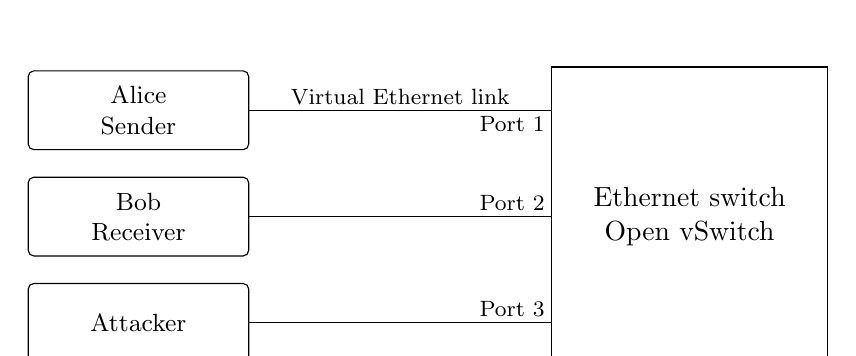
\begin{tikzpicture}
\node[host] (a) at (0,1.35) {Alice\\Sender};
\node[host] (b) at (0,0) {Bob\\Receiver};
\node[host] (x) at (0,-1.35) {Attacker};
\node[draw,minimum width=35mm,minimum height=38mm,align=center] (s) at (7,0) {Ethernet switch\\Open vSwitch};
\draw (a.east)--node[lab,above]{Virtual Ethernet link} ($(s.west)+(0,1.35)$) node[lab,pos=.87,below]{Port 1};
\draw (b.east)--($(s.west)+(0,0)$) node[lab,pos=.87,above]{Port 2};
\draw (x.east)--($(s.west)+(0,-1.35)$) node[lab,pos=.87,above]{Port 3};
\end{tikzpicture}
\caption{Implemented topology: one dedicated switch port per host, isolated from any external network.}\label{fig:topology}
\end{figure}

\subsection{Switching Environment}
The switch is a separately built Open vSwitch 3.3.9 instance, kept entirely apart from any system-installed switching service. Its eviction routine was fixed to a single, unconditional global oldest-dynamic-entry policy for every trial, so that the two compared cases differ only in whether the embedded fair-eviction controller runs before that base policy is ever invoked. Table~\ref{tab:config} lists the parameters held fixed across every trial reported in this document, exactly as adopted in the design report.

\begin{table}[H]
\centering
\begin{tabularx}{\linewidth}{@{}p{58mm}Y@{}}
\toprule
Parameter & Value\\\midrule
Forwarding-table capacity & 64 entries (dynamic and static combined)\\
Aging interval & 300 seconds\\
Switch ports & 3 (Alice, Bob, attacker), no VLAN segmentation\\
Flooding-frame count & 256 distinct false source addresses\\
Flooding nominal rate & 200 frames/second\\
Observation frames per stage & 10\\
Ethernet frame length & 60 bytes, excluding the frame check sequence\\
EtherType & \texttt{0x88B5}\\
Forwarding rule installed & Normal destination-based forwarding only, on every port\\\bottomrule
\end{tabularx}
\caption{Fixed configuration used for every trial in this report.}\label{tab:config}
\end{table}

\subsection{Frame Structure}
Frames were constructed and parsed exactly as specified in the design report (Figure~\ref{fig:frame}): a 6-byte destination address, a 6-byte source address, the 2-byte \texttt{0x88B5} EtherType, and 46 bytes of payload and zero padding, giving 60 bytes excluding the frame check sequence.

\begin{figure}[H]
\centering
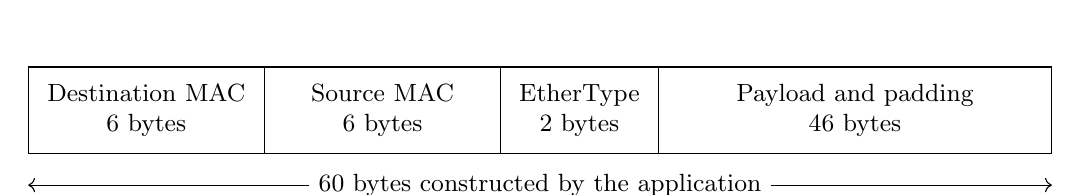
\begin{tikzpicture}[x=1cm]
\foreach \a/\b/\t/\s in {0/3/Destination MAC/6 bytes,3/6/Source MAC/6 bytes,6/8/EtherType/2 bytes,8/13/Payload and padding/46 bytes}{
\draw (\a,0) rectangle (\b,1.1);
\node[align=center,font=\small] at ({(\a+\b)/2},.55) {\t\\\s};}
\draw[<->] (0,-.4)--node[fill=white,font=\small]{60 bytes constructed by the application}(13,-.4);
\end{tikzpicture}
\caption{Implemented Ethernet frame layout (field widths schematic).}\label{fig:frame}
\end{figure}

Host addresses are the locally administered unicast values \texttt{02:40:06:00:00:01} (Alice), \texttt{02:40:06:00:00:02} (Bob), and \texttt{02:40:06:00:00:03} (attacker). False flooding sources use the prefix \texttt{02:FA} followed by a four-byte sequence number, giving 256 distinct, non-overlapping addresses. Flooding frames carry a distinct label and sequence number with a fixed destination of Alice; observation frames carry a separate label and sequence number with Alice as source and Bob as destination. No implementation detail of this frame layout changed between design and completion.

\section{Assumptions}\label{sec:assumptions}
Each host occupies a dedicated switch port with no other device sharing it, and Bob remains silent throughout flooding and the subsequent observation stage, so capacity-driven displacement, rather than ordinary source refreshing, is what determines whether his entry survives. No other legitimate traffic exists on the network during a trial beyond the defined learning and observation frames.

The table capacity (64 entries) and aging interval (300 seconds) are deliberately small configuration choices that make capacity exhaustion observable within seconds, not claims about typical production values; every trial completes well inside the aging interval, so displacement is attributable to capacity pressure rather than ordinary entry expiry. The switching environment is a software switch running in userspace mode, used as a stand-in for a hardware switch's learning and forwarding behaviour. Because eviction and counting are deterministic given a fixed sequence of learned addresses, one trial per configuration is treated as representative of that configuration rather than as one sample from a noisy process.

\section{Testing Methodology}\label{sec:testing}
Two complementary procedures were used throughout. Both instantiate a completely fresh switch instance and fresh host namespaces for every case, so neither case inherits forwarding state from the other, and both retain the same fixed global base eviction policy; only the embedded controller is toggled.

\textbf{Standard demonstration.} For each of the two cases (controller disabled, controller enabled), the procedure (i) sends one learning frame from each host, (ii) sends ten observation frames from Alice to Bob and captures at Bob and the attacker (\emph{baseline}), (iii) sends 256 flooding frames at a nominal 200 frames/second while capturing every flooding frame at Alice to verify wire-level delivery, (iv) with Bob still silent, repeats the ten observation frames and captures again (\emph{after flooding}), (v) lets Bob transmit one recovery learning frame, and (vi) repeats the ten observation frames once more (\emph{recovery}). Receiving sockets are started and confirmed ready before any traffic is sent, and every capture is matched against the exact expected source, destination, EtherType, and label rather than by count alone. Every trial in this report passed all associated automated validation checks (forwarding-table snapshots, sequence completeness, frame-header structure, port and address assignment, completion before the aging interval, and the exact expected eviction attribution); none failed.

\textbf{Attack-volume sweep.} To locate the exact point at which flooding becomes able to displace Bob, the same procedure was repeated with the flooding-frame count varied over $\{0,16,32,60,61,62,64,128,256\}$, once for each case, keeping every other parameter in Table~\ref{tab:config} fixed. Because eviction in this switch is a deterministic function of table occupancy and learning order rather than of any random process, one trial per configuration was sufficient to obtain a stable, exactly reproducible outcome at each point; this is noted on every figure derived from the sweep. Exposure is reported as the percentage of the ten post-flooding observation frames that the attacker received.

Both procedures record, at each stage, the exact captured frame bytes at every receiver, the full forwarding-table snapshot, and every eviction decision logged by the switch, so that every plotted number in this report traces back to a captured Ethernet frame or a table snapshot rather than to an assumption.

\section{Attack Results}
\subsection{Baseline, Attack, and Recovery Outcomes}
\begin{table}[H]
\centering
\begin{tabular}{@{}p{30mm}p{26mm}p{14mm}p{16mm}p{28mm}@{}}
\toprule
Case & Stage & Table entries & Bob's entry & Frames received (Bob / attacker)\\\midrule
Without defense & Baseline & 3 & Present & 10 / 0\\
Without defense & After flooding & 64 & \textbf{Absent} & 10 / \textbf{10}\\
Without defense & Recovery & 64 & Present & 10 / 0\\\midrule
With defense & Baseline & 3 & Present & 10 / 0\\
With defense & After flooding & 64 & Present & 10 / 0\\
With defense & Recovery & 64 & Present & 10 / 0\\\bottomrule
\end{tabular}
\caption{Measured outcome of the standard 256-address demonstration. Every row passed frame-level validation.}\label{tab:results}
\end{table}

\subsection{Traffic Timeline}
Figure~\ref{fig:timeline} plots every captured frame at its measured reception timestamp for one representative run of the standard demonstration, rather than only the aggregated counts in Table~\ref{tab:results}. It was produced by post-processing the exact per-frame capture timestamps recorded during that run, using the parameters in Table~\ref{tab:config}; no separate configuration was introduced for this figure.

\begin{figure}[H]
\centering
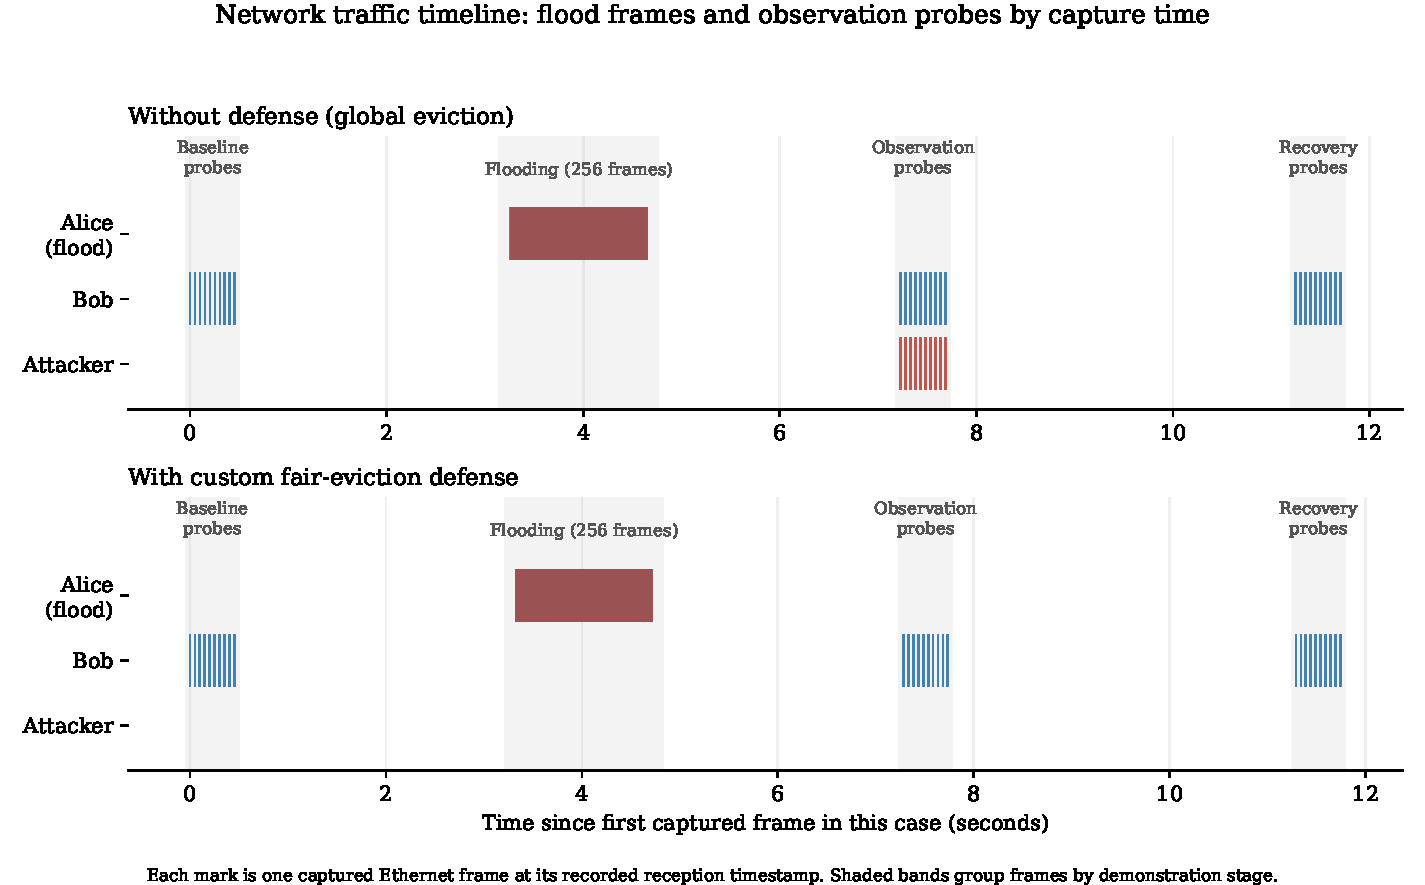
\includegraphics[width=\linewidth]{figures/network_traffic_timeline.pdf}
\caption{Captured Ethernet frames by reception time for the standard demonstration, without defense (top) and with defense (bottom). Each mark is one captured frame; shaded bands group frames by stage.}\label{fig:timeline}
\end{figure}

The flooding stage appears as a dense, near-continuous block on Alice's row, consistent with a sustained burst rather than isolated packets, and lasts a little over a second, consistent with 256 frames sent at a nominal 200 frames/second including per-frame pacing overhead. The observation stage that follows shows the attacker row populated only in the undefended case; the attacker's row is otherwise empty throughout its capture window in every other stage of both cases, which is the same conclusion Table~\ref{tab:results} reports, now visible directly as captured traffic rather than as a derived count.

\begin{figure}[H]
\centering
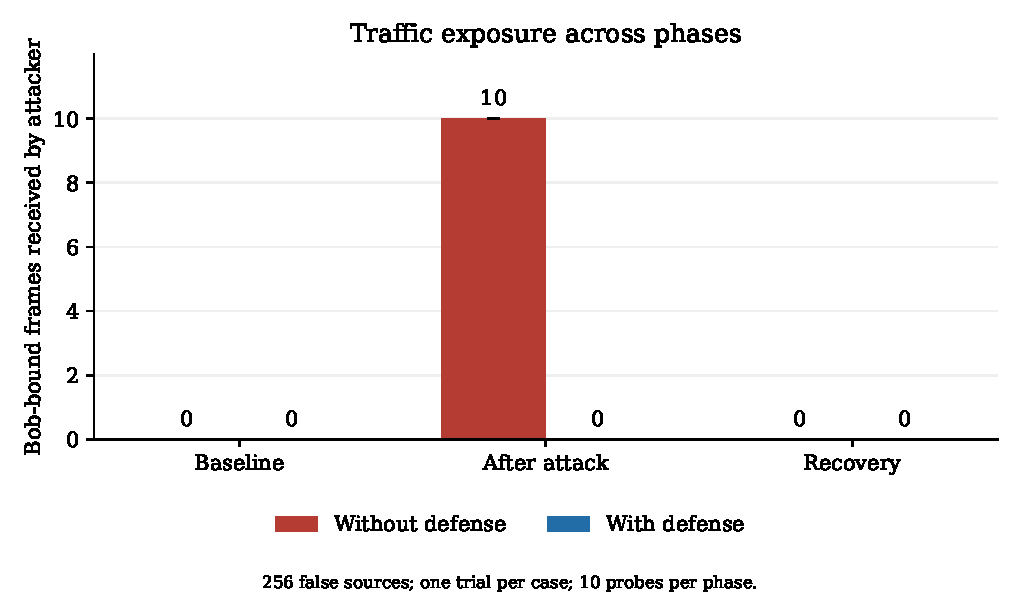
\includegraphics[width=.49\linewidth]{figures/traffic_exposure.pdf}\hfill
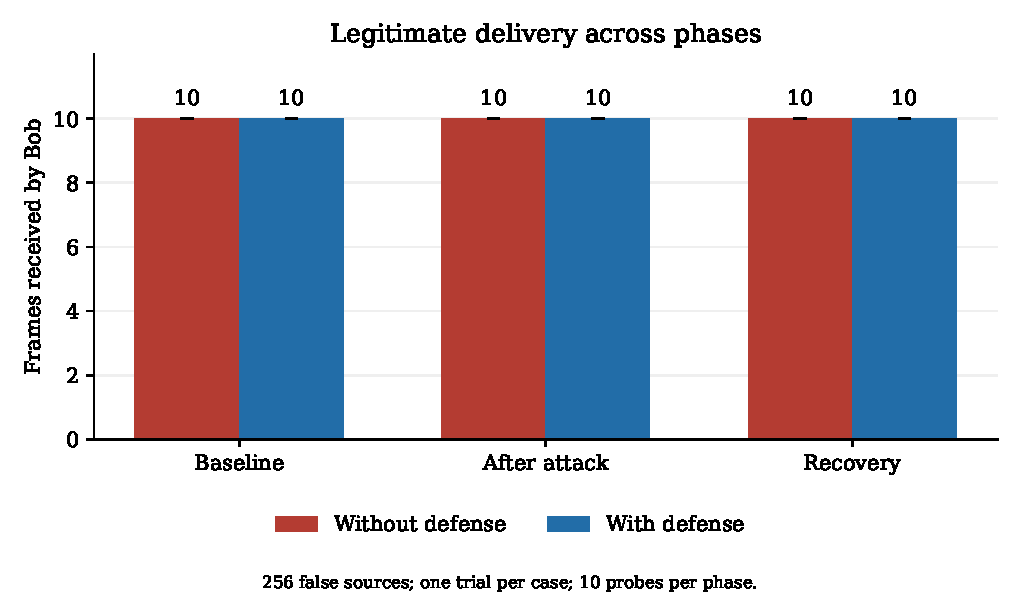
\includegraphics[width=.49\linewidth]{figures/legitimate_delivery.pdf}
\caption{Left: frames received by the attacker across stages at 256 flooding addresses. Right: frames received by Bob across the same stages. Configuration as in Table~\ref{tab:config}; single trial per stage and case.}\label{fig:phasebars}
\end{figure}

Figure~\ref{fig:phasebars} restates Table~\ref{tab:results} graphically: exposure at the attacker is zero in every stage except the undefended attack stage, while delivery to Bob is unaffected by either the attack or the defense in every stage. This separates two properties that are easy to conflate: the defense's effect is entirely on \emph{who else} receives Bob's traffic, not on whether Bob receives it.

\subsection{Sensitivity to Attack Volume}
Table~\ref{tab:config} fixes the flooding count at 256, well above the 64-entry capacity, but the design report's justification for the attack rests on capacity being exceeded, not on the specific number 256. The sweep described in Section~\ref{sec:testing} tests this directly.

\begin{figure}[H]
\centering
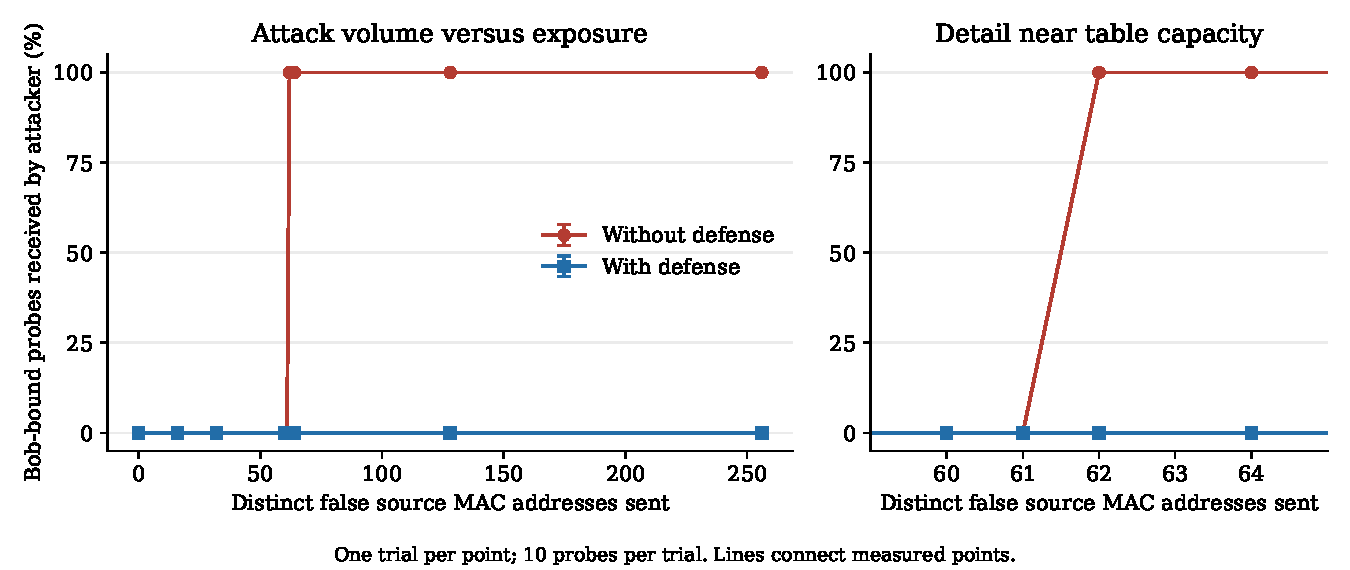
\includegraphics[width=\linewidth]{figures/attack_volume_vs_exposure.pdf}
\caption{Attacker-received percentage of the ten post-flooding observation frames, as a function of the number of distinct false source addresses sent, for both cases. Left: full range 0--256. Right: detail around the table's capacity boundary. One trial per point (see Section~\ref{sec:testing}); the outcome at each point is exactly reproducible under this deterministic eviction mechanism.}\label{fig:sweep}
\end{figure}

With three legitimate entries already learned before flooding begins, the table has exactly $64-3=61$ free positions. Exposure without the controller is 0\% for every tested volume up to and including 61 addresses and jumps to 100\% at 62 addresses and remains 100\% at every larger tested volume, an exact match to the free-capacity arithmetic rather than an approximate threshold. With the controller enabled, exposure stays at 0\% across the entire tested range, including volumes well beyond capacity, because the controller supplies free space from the attacker's own entries before the base global policy is ever invoked.

\begin{figure}[H]
\centering
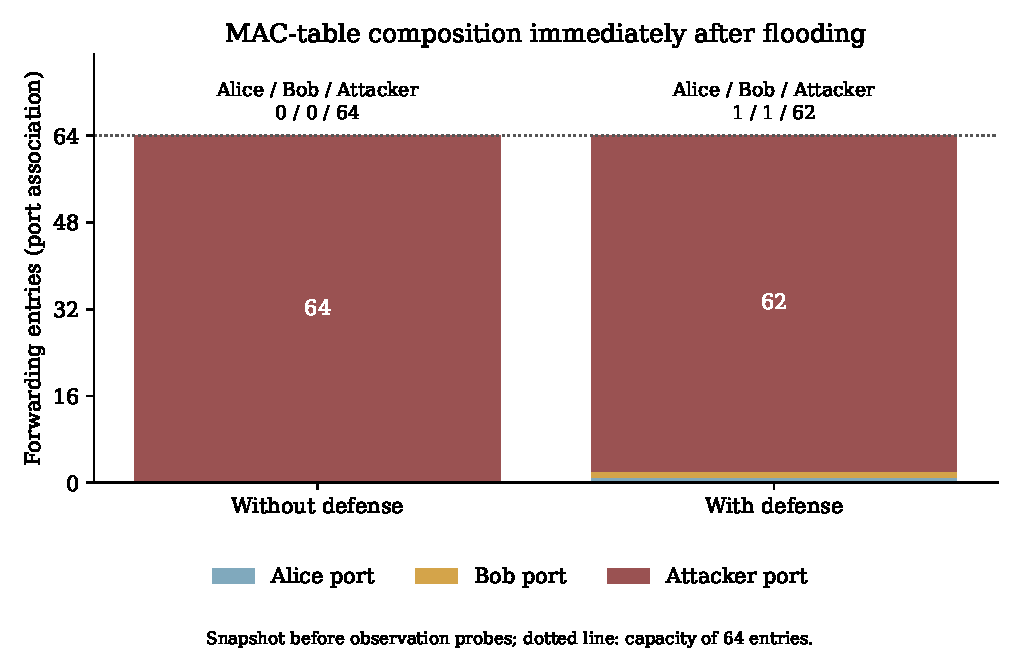
\includegraphics[width=.68\linewidth]{figures/mac_table_composition.pdf}
\caption{Forwarding-table composition by port, captured immediately after 256-address flooding and before the post-flood observation frames, for both cases. Dotted line: table capacity.}\label{fig:composition}
\end{figure}

Figure~\ref{fig:composition} explains the mechanism behind Figure~\ref{fig:sweep}: without the controller, the full table ends up occupied entirely by attacker-port entries, meaning Alice's and Bob's earlier entries were both evicted at some point during flooding; with the controller, Alice's and Bob's single entries each survive, and the attacker port accounts for all but two of the 64 entries. The controller made 195 eviction decisions during the 256-address flood, each removing one attacker-port entry immediately before the corresponding new false source was learned, consistent with $256+3-64=195$ required evictions once the table first reaches capacity. This same relationship held at every tested volume above capacity (1 eviction at 62 addresses, 3 at 64, 67 at 128, 195 at 256), and zero evictions were logged by the controller at or below 61 addresses, since no eviction is needed there.

\section{Defense Design}
The controller executes inside the switch's source-learning path, under the same write lock that already serializes table modifications, and runs before the base capacity check for every newly seen source address. It performs no action while free capacity remains. Once the table is full, it counts current dynamic entries by port and removes the least-recently-learned dynamic entry belonging to whichever port currently holds the most entries; the base global-eviction routine underneath it is never reached while the controller is active. Static entries are excluded from both counting and selection. Algorithm~\ref{alg:fair-eviction} restates this exactly as implemented.

\begin{algobox}{Fair-eviction controller (invoked before new-source insertion)}
\label{alg:fair-eviction}
\textbf{Input:} new source address $s$ on incoming port $p_{in}$; forwarding table $T$ with capacity $C$.
\begin{enumerate}
\item \textbf{If} $s$ already has an entry in $T$: update its source association and learning recency, and stop.
\item \textbf{If} $|T| = C$ (table full):
\begin{enumerate}
\item $p^{*} \leftarrow \textsc{null}$; $\mathit{count}_{\max} \leftarrow 0$.
\item \textbf{For each} eligible dynamic entry $e$ in $T$, taken oldest to newest:
\begin{enumerate}
\item $p \leftarrow \mathrm{port}(e)$; $\;c \leftarrow$ number of entries in $T$ currently on port $p$.
\item \textbf{If} $c > \mathit{count}_{\max}$: set $\mathit{count}_{\max} \leftarrow c$ and $p^{*} \leftarrow p$.
\end{enumerate}
\item Remove the oldest eligible dynamic entry belonging to port $p^{*}$ from $T$.
\end{enumerate}
\item Insert the new entry $(s, p_{in})$ into $T$.
\end{enumerate}
\end{algobox}

Because Alice and Bob each contribute exactly one entry while the attacker contributes up to 256, the attacker's port is the largest contributor from the very first eviction onward in every trial reported here, so every eviction removes an attacker-owned entry and Alice's and Bob's entries are never candidates once at least one other port holds more entries than they do.

\section{Expected versus Observed Outcomes}
Table~\ref{tab:expected} compares the outcomes anticipated in the design report against what was actually measured.

\begin{table}[H]
\centering
\footnotesize
\begin{tabular}{@{}ll@{}}
\toprule
Expected (design report) & Observed\\\midrule
Global eviction displaces Bob at capacity & 0\% exposure up to 61 addresses, 100\% at 62+\\
Bob still receives traffic while exposed & 10 of 10 in every stage\\
Attacker's port is evicted first by the controller & 100\% of controller evictions were attacker-owned\\
Controller prevents exposure generally, not only at 256 & 0\% exposure across the entire swept range\\
Recovery restores private delivery & Confirmed in both cases\\\bottomrule
\end{tabular}
\caption{Design-time expectations against measured results.}\label{tab:expected}
\end{table}

No expectation was contradicted; the sweep in Section~\ref{sec:testing} refines the qualitative prediction into an exact capacity boundary.

\section{Limitations}\label{sec:limitations}
\subsection{Limitations of the Attack}
Bob was kept completely silent throughout the attack. A device that keeps sending traffic refreshes its own entry, so a more active victim might not have been evicted at all. The impact measured here is that Bob's traffic gets copied to the attacker, not that it stops reaching Bob: no delivery was blocked in any trial. Finally, every false address came from a single attacker port; spreading the same addresses across several ports was not tried and could behave differently.

\subsection{Limitations of the Defense}
The controller protects a port's fair share of the table, not the identity of any address; it never checks whether a source is genuine. If devices share a port, or if the balance of entries shifts, including across several attacker-controlled ports, a legitimate entry could still end up being the one removed. Splitting the same flood across multiple ports, so that no single port stands out, was not tried here. The controller also keeps counting and evicting for as long as the flood continues, so it still costs the switch ongoing work rather than stopping the flood outright. Protecting specific addresses and capping how many a single port can register were both considered but were not built into this defense. Everything reported here comes from one fixed setup, three ports and a 64-entry table; larger tables or different topologies were not tested.

\section{Conclusion}
The implementation reproduced every qualitative outcome anticipated in the design report and additionally located the exact capacity boundary at which the undefended attack succeeds, confirming it matches the table's free capacity rather than an approximate threshold. The embedded fair-eviction controller held attacker exposure at zero across the entire tested range of attack volumes while leaving legitimate delivery to Bob unaffected in every stage of every trial, at the cost of the specific assumptions and limitations enumerated in Sections~\ref{sec:assumptions} and~\ref{sec:limitations}. These results support treating table-composition-aware eviction as an effective, narrowly scoped mitigation for this class of exposure, rather than as a complete defense against MAC table flooding in general.

\section{Group Responsibilities}
\begin{center}
\begin{tabular}{@{}ll@{}}
\toprule Student ID & Responsibility\\\midrule
2105085 & Attack implementation, attack-side testing and result analysis\\
2105062 & Defense implementation, defense-side testing and result analysis\\\bottomrule
\end{tabular}
\end{center}
\end{document}
